\documentclass[11pt,a4paper]{article}
\usepackage[english]{babel}
\usepackage[letterpaper,top=2cm,bottom=2cm,left=3cm,right=3cm,marginparwidth=1.75cm]{geometry}
\usepackage{amsmath}
\usepackage{amsfonts} 
\usepackage{graphicx}
\usepackage{url}
\usepackage{float}

\DeclareMathOperator{\atantwo}{atan2}

\title{Image-based Trajectory Determination of Artificial Satellites \\\large State of the art, performance comparison and critical assessment}
\author{Frederic Heil\\
	\texttt{frederic.heil@hs-weingarten.de}\\
	\textbf{Ravensburg-Weingarten University of Applied Sciences}
}
\date{October 15, 2026}

\begin{document}
	\maketitle
	
	\section{Introduction}
	
	Previously, the preliminary paper established underlying geometric fundamentals and four methods for orbit determination: two based on a single-camera and two on a dual-camera setup, with one method in each setup determining circular orbits and the other full orbital parameters. The research paper continued with experimental setups to evaluate how these methods react to variable parameters, star-based calibration and different satellite altitudes. The aim of this concluding paper is to contextualize results into the state of art and compare accuracies. Additionally, certain issues of methods need to be assessed. Lastly, we aim to conclude which methods retain their practical use-case in the scope of image-based orbit determination with short observation arcs.
	
	\section{State of the art}
	\section{Performance comparison}
	\section{Critical assessment}
	\subsection{Observation difficulties in real world settings}
	Previously, the research paper established an experimental setup on how the orbit determination methods can be subjected to variable parameters to evaluate their accuracy under different conditions. Results indicate, that  methods which do not compromise on a circular model, require long observation arcs $\Delta \theta$ \cite{orbit_determination_research} as pictured below in figure \ref{fig:sma_errors_full_single}.
	
	\begin{figure}[H]
		\centering
		\begin{minipage}{0.49\textwidth}
			\centering
			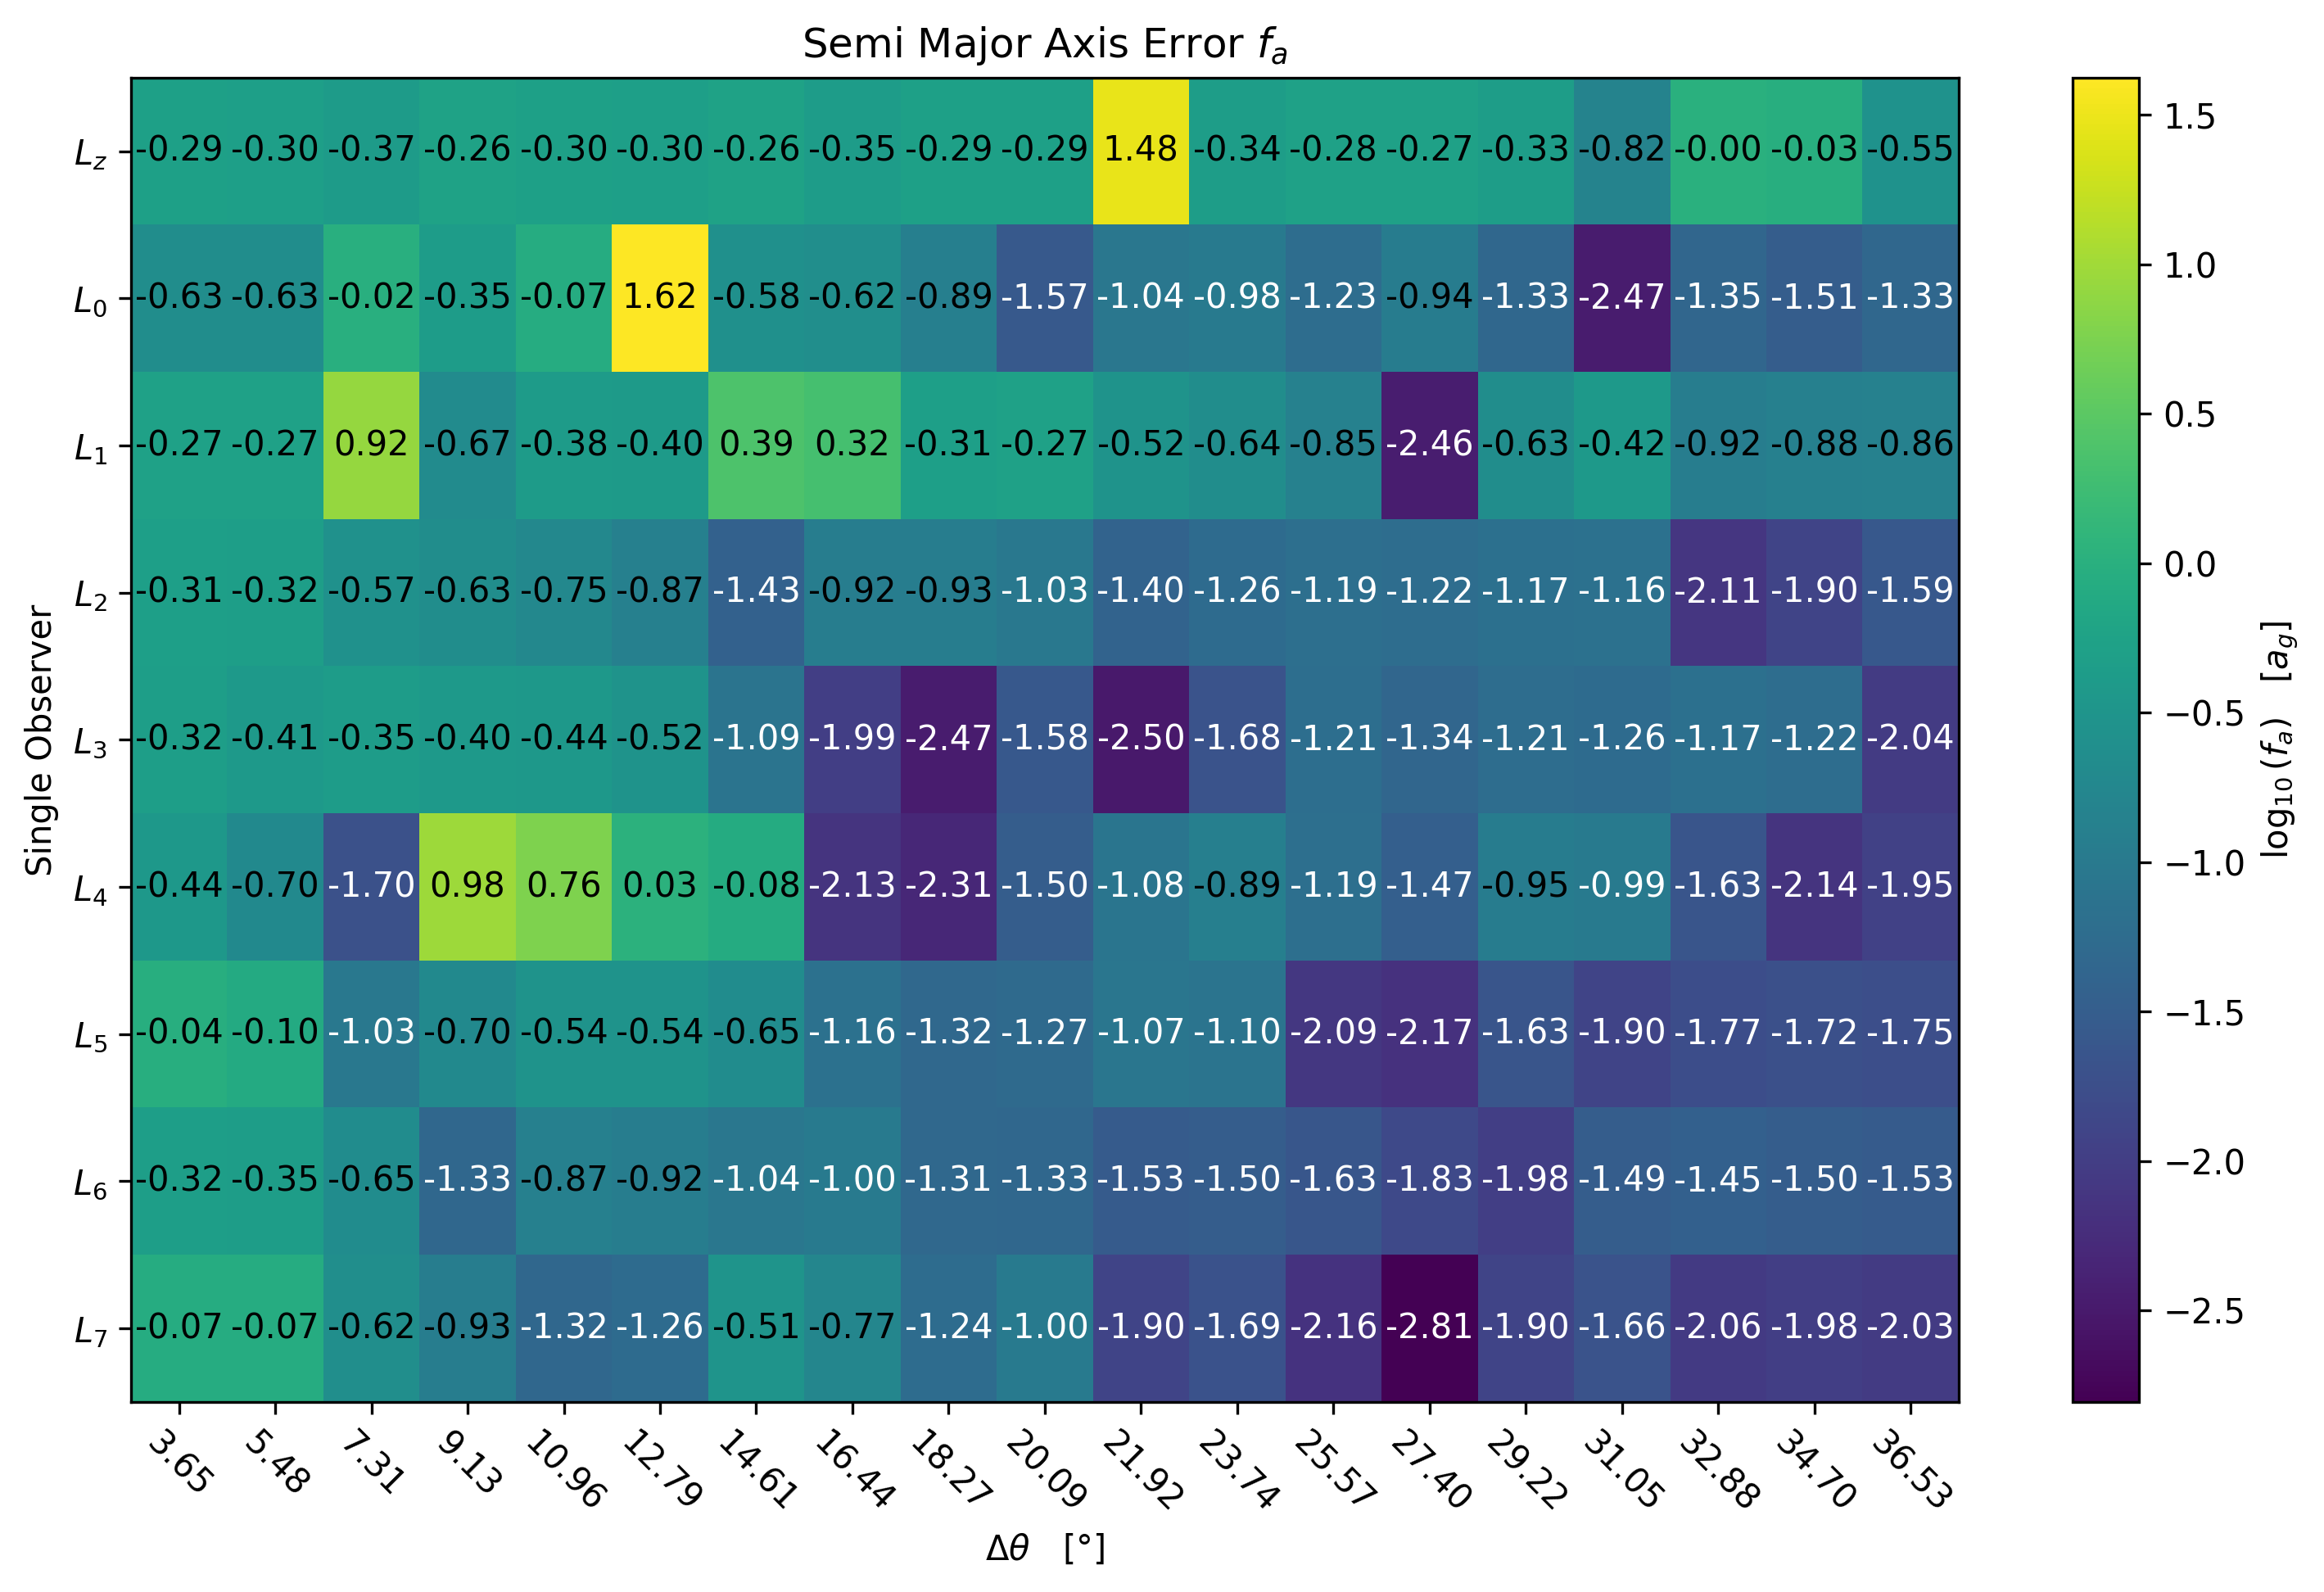
\includegraphics[width=\linewidth]{plots/sma_errors_full_single.png}
			\caption{Gaussian method requiring large $\Delta \theta$ for reasonable parameter prediction \cite{orbit_determination_research}.}
			\label{fig:sma_errors_full_single}
		\end{minipage}
		\hfill
		\begin{minipage}{0.49\textwidth}
			\centering
			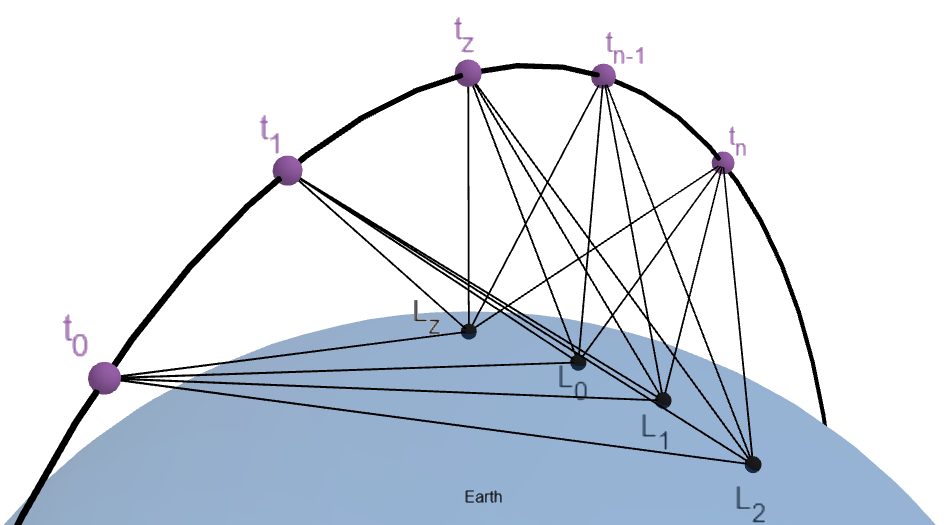
\includegraphics[width=\linewidth]{images/observation_schematic.png}
			\caption{Schematic of strategic camera placement \cite{orbit_determination_research}.}
			\label{fig:observation_schematic}
		\end{minipage}
	\end{figure}
	\noindent
	Figure \ref{fig:observation_schematic} illustrates 
	
	
	
	- observation span
	- atmospheric interference close to horizon
	- clouds
	- satellite illumination, (dämmerlicht)
	\subsection{Numerical instability of the Gaussian method}
	Mentioned previously, the research paper suggests that the Gaussian method contains a numerical instability for observations from observer location $L_z$ or close \cite{orbit_determination_research} as visible in figure \ref{fig:sma_errors_full_single} where semi major axes tend to be predicted more reliably the further the observer is located from the orbital plane.
	After close inspection, this issue seems to arise from the $D_0$ scalar, or rather a set of equations as part of the algorithm, where
	
	\begin{equation*}
		D_0=v_1\cdot m_1 \quad\text{with}\quad m_1=v_2\times v_3
	\end{equation*}
	gets inserted into
	
	\begin{equation*}
		\begin{aligned}
			A = \frac{1}{D_0}
			\left(
			-D_{12}\frac{\tau_3}{\tau}
			+ D_{22}
			+ D_{32}\frac{\tau_1}{\tau}
			\right) \\
			B = \frac{1}{6D_0}
			\left(
			D_{12}\left(\tau_3^2-\tau^2\right)\frac{\tau_3}{\tau}
			+
			D_{32}\left(\tau^2-\tau_1^2\right)\frac{\tau_1}{\tau}
			\right)
		\end{aligned}
	\end{equation*}
	\cite{curtis_gauss_algo}
	
	\subsection{Weakness of the simplified Gaussian method}
	The simplified Gaussian method assumes a circular orbit by default. Research results have shown, that it is quite accurate in predicting a satellite's trajectory within seconds if the underlying ground truth orbit is also circular \cite{orbit_determination_research}. Issues arise if the underlying ground truth orbit is elliptical which is investigated in this section. First, we recapitulate one of the initial ideas it is based upon, namely the relation between recorded time stamps and orbital period:
	
	\begin{equation}
		\label{circle_gauss_delta_t}
		t_2 - t_1 = \Delta t=\frac{\varphi}{2\pi}T
	\end{equation} 
	\newline
	Hereby, $\varphi$ equates the angle of an arc which the satellite traverses between $t_1$ and $t_2$. \cite{orbit_determination_preliminary}\newline In other places we use $\Delta \theta$ to describe the passage angle. We insert $\Delta \theta$ for $\varphi$ and reformulate equation \ref{circle_gauss_delta_t} as follows:
	
	\begin{equation*}
		\Delta t=\frac{\Delta \theta}{2\pi}T \Leftrightarrow \frac{2\pi}{T}=\frac{\Delta \theta}{\Delta t}=\omega
	\end{equation*}
	We obtain $\frac{\Delta \theta}{\Delta t}$, an angular velocity value $\omega$ (not to be confused with argument of periapsis). Furthermore, it is trivially known that circular trajectory velocity $v$ relates to angular velocity in scalar-notation as follows:
	
	\begin{equation}
		v = \omega \cdot r_{\perp} \Leftrightarrow \omega = \frac{v}{r_{\perp}}
	\end{equation}
	This relation holds if the velocity vector is perpendicular to the radius vector, thus at every position for circular trajectories. Regarding elliptical trajectories, this relation without modification only holds at periapsis and apoapsis which is sufficient for our purposes.\newline
	Next, Weber provides the \emph{Vis Viva} equation, which describes current velocity $v$ subject to current radius $r$ of an object moving along an elliptical trajectory with given semi major axis $a$ as follows:
	
	\begin{equation}
		\label{vis_viva}
		v=\sqrt{\mu\left(\frac{2}{r}-\frac{1}{a}\right)}
	\end{equation}
	\cite{hohmann_transfer}\newline
	This equation can be reformulated as angular velocity
	\begin{equation}
		\label{vis_viva_angular}
		\omega=\frac{\sqrt{\mu\left(\frac{2}{r_{\perp}}-\frac{1}{a}\right)}}{r_{\perp}}
	\end{equation}
	which holds for $r_{\perp}\in\{a, r_{pe}, r_{ap}\}$. Suppose that the simplified Gaussian method is applied to a satellite on an elliptical trajectory, located at its trajectory's periapsis or apoapsis, we can now determine what semi major axis $a_m$ will be predicted from ground truth semi major axis $a_g$ subject to eccentricity $0 \leq e < 1$.\newline
	The approach is to equate $\ref{vis_viva_angular}$ with itself for $r_{\perp}=r_{pe/ap}$, $a=a_g$ and $r_{\perp}=a_m$, $a=a_m$ and rephrase it to obtain $a_m$. Hence:
	
	\begin{equation*}
		\begin{aligned}
			\frac{\sqrt{\mu\left(\frac{2}{r_{pe/ap}}-\frac{1}{a_g}\right)}}{r_{pe/ap}} = \frac{\sqrt{\mu\left(\frac{2}{a_m}-\frac{1}{a_m}\right)}}{a_m} \Leftrightarrow \\
			\frac{\sqrt{\left(\frac{2}{r_{pe/ap}}-\frac{1}{a_g}\right)}}{r_{pe/ap}} = 
			(a_m^{-1})^{\frac{1}{2}}\cdot a_m^{-1}=a_m^{-\frac{3}{2}} \Leftrightarrow \\
			\left(\frac{\sqrt{\left(\frac{2}{r_{pe/ap}}-\frac{1}{a_g}\right)}}{r_{pe/ap}}\right)^{-\frac{2}{3}}=a_m
		\end{aligned}
	\end{equation*}
	It is trivially known that $r_{pe/ap}=a(1\mp e)$, hence we insert this term to obtain $a_{m(pe/ap)}$ subject to $e$:
	\begin{equation*}
		a_{m(pe/ap)}=\left(\frac{\sqrt{\left(\frac{2}{a_g(1\mp e)}-\frac{1}{a_g}\right)}}{a_g(1\mp e)}\right)^{-\frac{2}{3}} = \frac{a_g(1\mp e)}{\sqrt[3]{1\pm e}}
	\end{equation*}
	Thus:
	\begin{equation}
		\label{predicted_sma_subject_to_ecc}
		\boxed{a_{m(pe/ap)} = \frac{a_g(1\mp e)}{\sqrt[3]{1\pm e}}	}	
	\end{equation}
	This formula yields the values which the simplified Gaussian method would determine for measurements at periapsis and apoapsis. It works under the assumption that $\Delta t$ is short, meaning no significant change in $\omega$ between recordings.
	
	\begin{figure}[H]
		\centering
		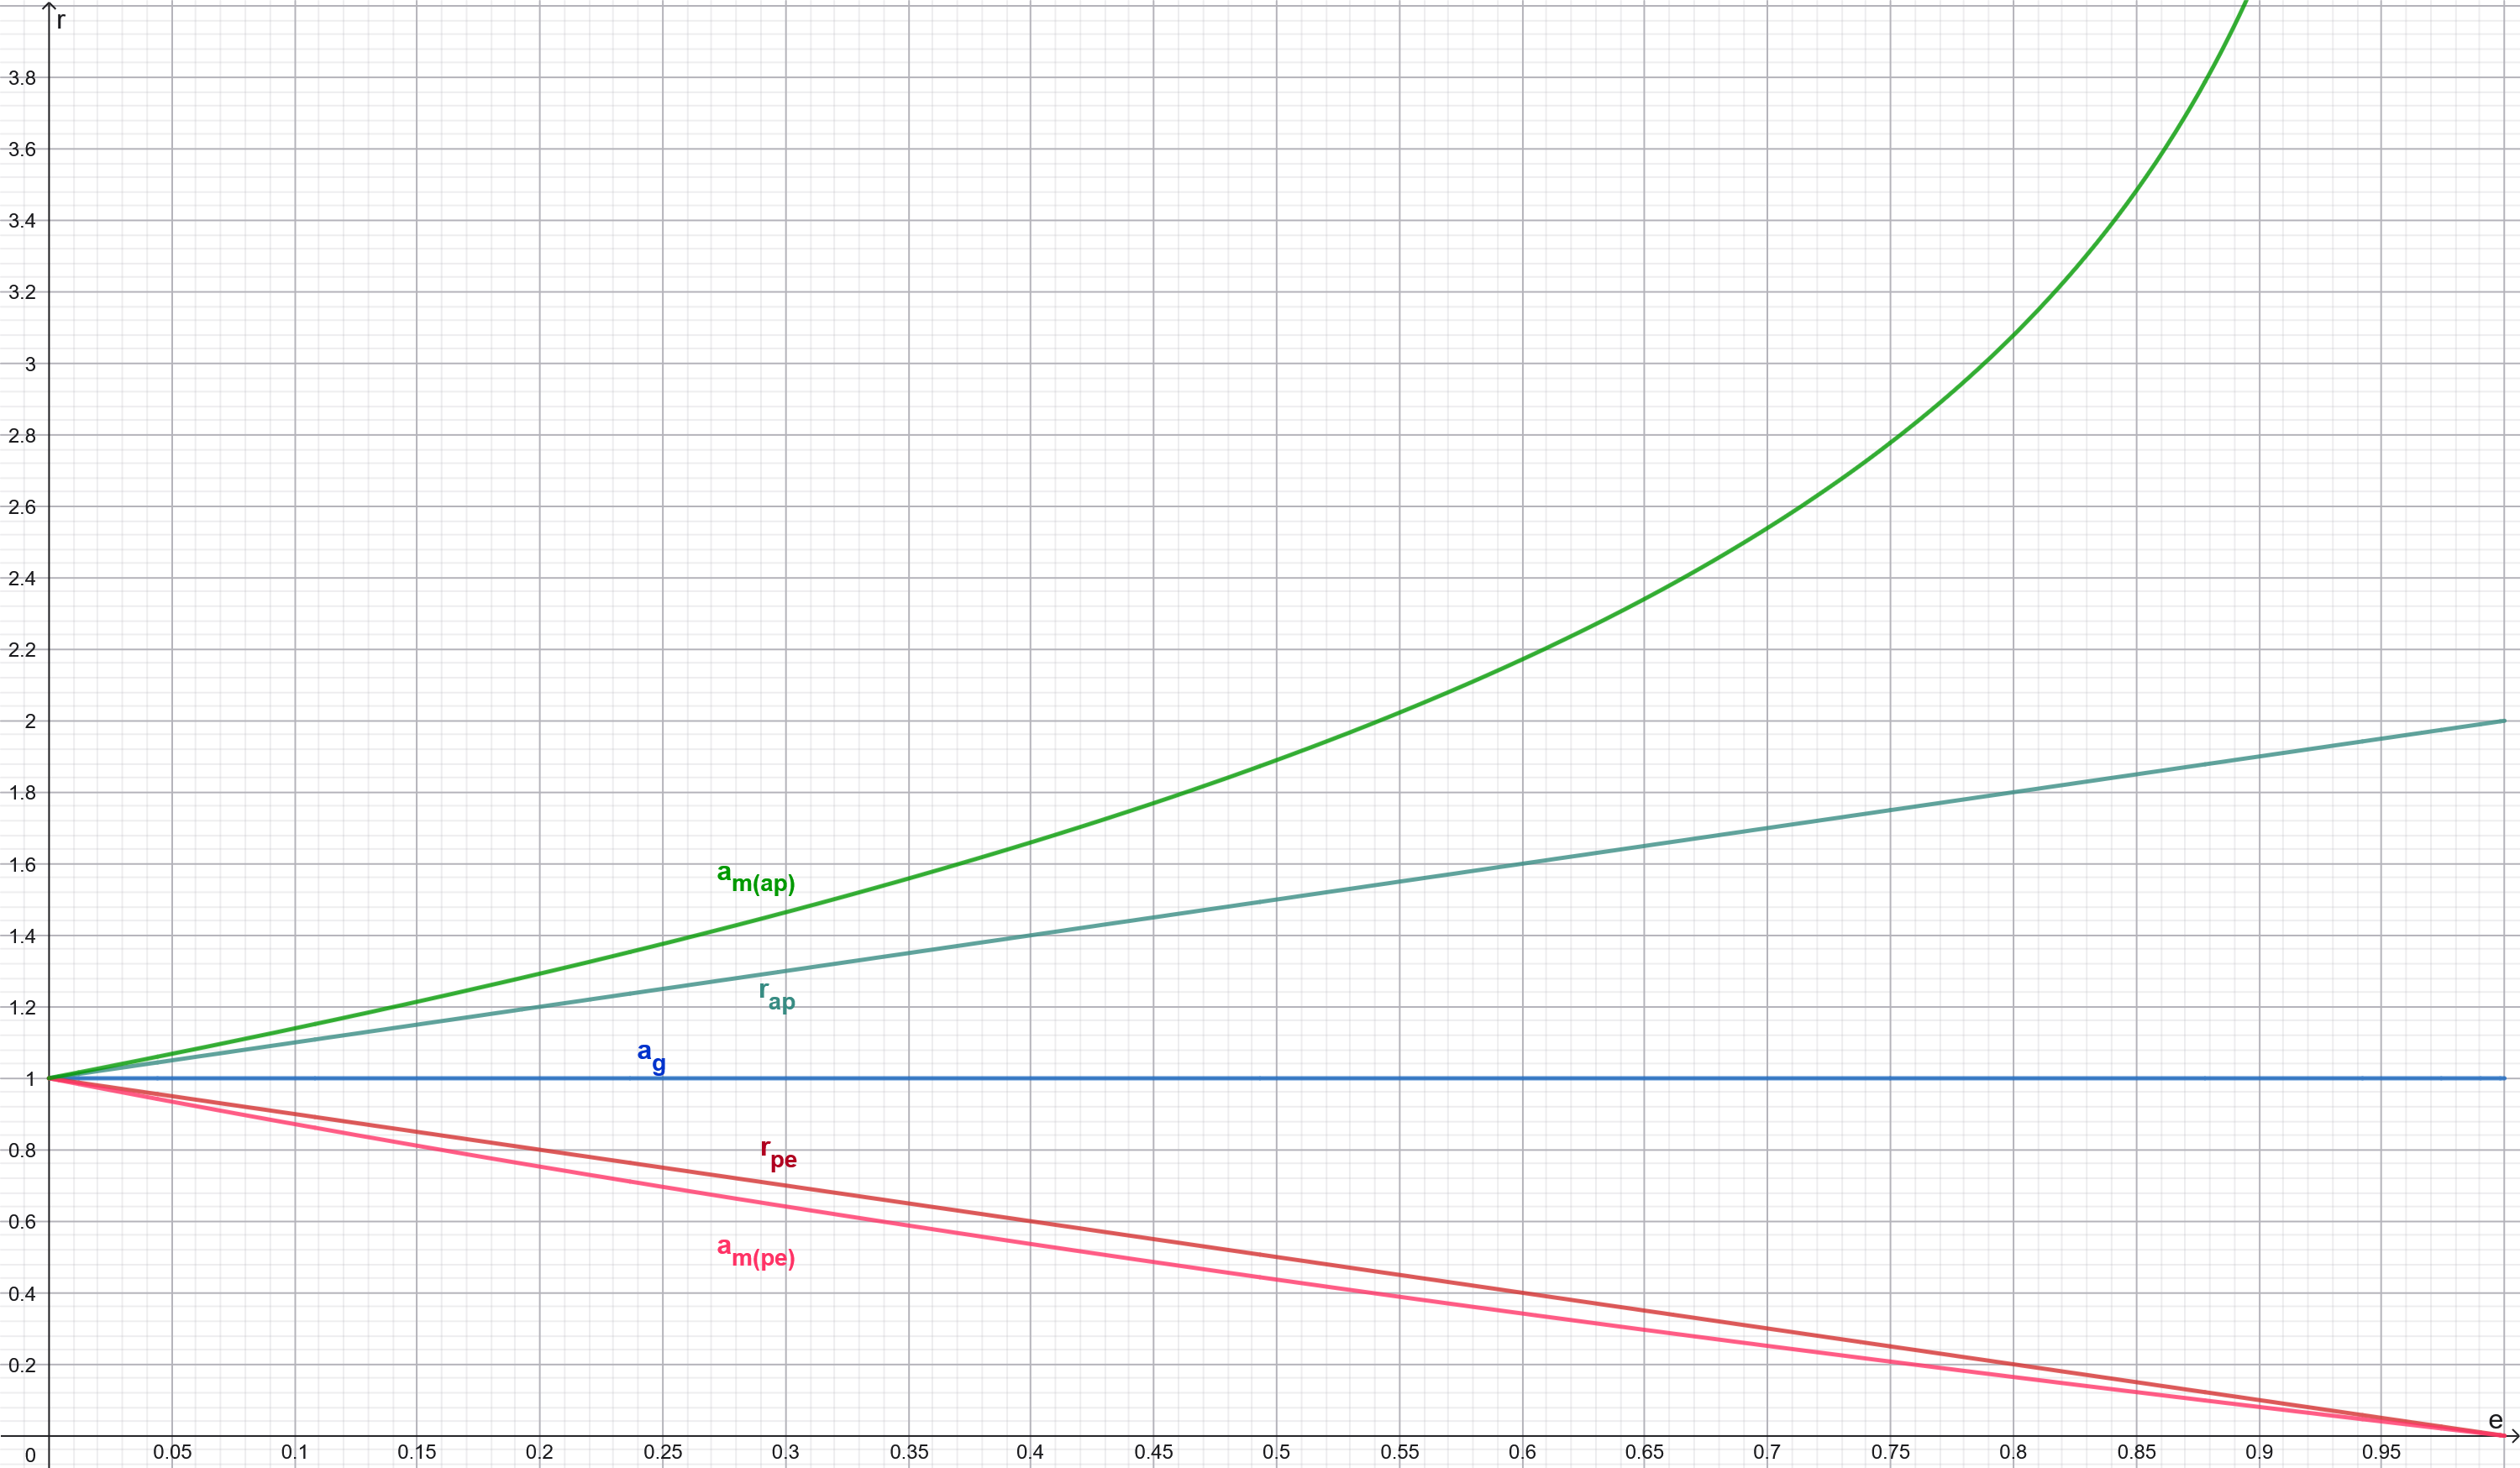
\includegraphics[width=1.0\linewidth]{images/sg_instability.png}
		\caption{Predicted semi major axis values $a_p$ if measurements were conducted at periapsis or apoapsis subject to eccentricity $e$. }
		\label{fig:error_propagation_schematic}
	\end{figure}
	\noindent
	Pictured above are curves of periapsis and apoapsis radii $r_{pe}$ and $r_{ap}$ and predicted semi major axes $a_{m(pe)}$ and $a_{m(ap)}$ subject to eccentricity $0 \leq e < 1$ for generic ground truth semi major axis $a_g=1$ as output of equation \ref{predicted_sma_subject_to_ecc}.\newline 
	We observe that, when measured and applied at periapsis, predicted semi major axes lie even below $r_{pe}$, meaning that the predicted circular orbits would lie completely within the elliptical ground truth orbit. As for measurements at apoapsis, we observe that predicted semi major axes lie above $r_{ap}$ with growing tendency as $e$ increases. This means that the ground truth elliptical orbit lies completely within predicted circular orbits.\newline
	Predicted semi major axes from other positions than periapsis or apoapsis, which is the average case, would lie in between these values and might be a closer match to $a_g$. However, this approach shows how far predictions might deviate from reality under poor circumstances, highlighting the potential instability of the simplified Gaussian method, rendering it suitable for near perfect circular orbits only.
	
	
	\section{Conclusion}
	
	
	\newpage
	\begin{thebibliography}{9}
		\setlength{\itemsep}{4pt}       % space between bibliography items
		\setlength{\parskip}{0pt}       % space between paragraphs
		\setlength{\parsep}{0pt}        % extra space within items
		
		
		
		\bibitem{semi_major_axis_knowledge}
		Carpenter, J.R. and Schiesser, E.R. (2001):
		\emph{Semi-Major Axis Knowledge and GPS Orbit Determination}.
		In: \emph{Journal of the Institute of Navigation}, 48(1).
		\newline
		\url{https://ntrs.nasa.gov/citations/20000084327}
		\newline
		Accessed: 2026-10-09
		
		\bibitem{orbit_determination_preliminary} Heil, F. (2026): \emph{Image based trajectory determination of artificial satellites}. \newline \url{https://github.com/stonkchonk/satellite-trajectories/blob/main/thesis/preliminary.pdf} \newline Accessed: 2026-10-11
		
		\bibitem{orbit_determination_research}
		Heil, F. (2026): \emph{Performance Comparison of Single- and Dual-Camera Setups for Image-Based Satellite Orbit Determination}.
		\newline
		\url{https://github.com/stonkchonk/satellite-trajectories/blob/main/thesis/research.pdf}
		\newline
		Accessed: 2026-10-11
		
		\bibitem{curtis_gauss_algo} Curtis, H.D. (2010): \emph{Gauss method of preliminary orbit determination}. In: \emph{Orbital Mechanics for Engineering Students}, 2nd ed., pp. 297--304. \newline \url{https://shop.elsevier.com/books/orbital-mechanics-for-engineering-students/curtis/978-0-12-374778-5} \newline Accessed: 2026-05-03 
	
		
		\bibitem{hohmann_transfer}
		Weber, B. (n.d.): \emph{Hohmann Transfer}.
		Orbital Mechanics \& Astrodynamics.
		\newline
		\url{https://orbital-mechanics.space/orbital-maneuvers/hohmann-transfer.html}
		\newline
		Accessed: 2026-10-12
	\end{thebibliography}
\end{document}